%--------------------------------------------------------------------------------------
% Este arquivo contém a sua metodologia
%--------------------------------------------------------------------------------------
\chapter{Materiais e Métodos} \label{ch:MM} %Uma label é como você referencia uma seção no texto com a tag \ref{}


\section{Arquitetura do Sistema embarcado do foguete} 

Com o intuito de capturar as principais grandezas produzidas pelo minifoguete e reduzir a massa e o volume ocupado pelo sistema, foi escolhido sensores capazes de mensurar mais de uma variável em um único encapsulamento e assim reduzir a necessidade de vários sensores separados. 

O microcontrolador foi escolhido tomando como base um custo-benefício melhor do que o atmega328p, que é bastante popular na plataforma arduino. Na data 05/04/2022, esse microcontrolador pode ser encontrado na loja Aliexpress por $47,31$ reais, já o STM32f103C8T6 por $36,47$. Além da redução de custo, o microcontrolador escolhido apresenta dez vezes mais memória SRAM, mais periféricos, processamento em $32 \ bits$ contra $8 \ bits$ e execução das instruções com clock de $72 \ MHz$ contra $16 \ MHz$ do atmega328p. 

Por fim, o rádio selecionado foi o modulo Lora, por apresentar um baixo custo e possuir um longo alcance de até $8 \ km$, possibilitando assim, seu uso em minifoguetes avançados. Com esses componentes escolhidos, foi projetado o diagrama mostrado na figura \ref{fig:Fluxograma_Sistema1}, que representa um sistema simples de entrada de dados através dos sensores, pre-processamento desses dados pelo microcontrolador e por fim a saída através da gravação em um cartão micro SD e o envio pelo rádio.



 


\begin{figure}[ht]
    \centering
    \caption{Diagrama sistema embarcado do minifoguete.}
    \begin{center}
        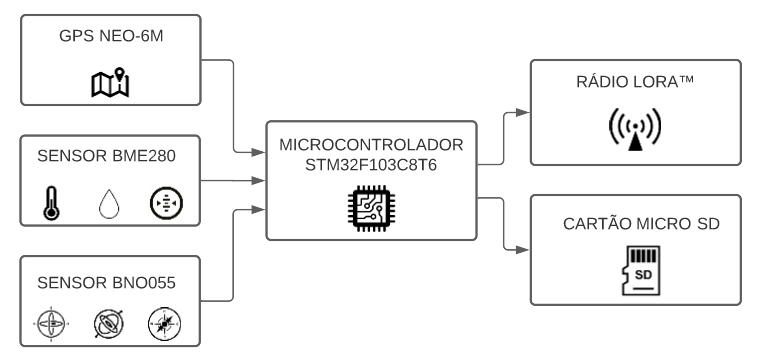
\includegraphics[width=1.0\textwidth]{img/Fluxograma_Sistema1.png}
    \end{center}
    \vspace{-0.5cm}
    \legend{\ABNTEXfontereduzida \textbf{Fonte: O autor.}}
    %\citeonline{BNO055}.}
    \label{fig:Fluxograma_Sistema1}
\end{figure}.





\section{Arquitetura do Sistema embarcado receptor } 

O sistema receptor é mais simples do que o sistema transmissor contido no foguete, porque, a única função desse sistema é repassar os dados recebidos do foguete para o computador. Como mostra o diagrama da figura \ref{fig:Fluxograma_Sistema2}, esse sistema possui apenas um modulo de rádio Lora na configuração receptor e um microcontrolador responsável por comunicar com o computador.





 



\begin{figure}[ht]
    \centering
    \caption{Diagrama sistema em solo.}
    \begin{center}
        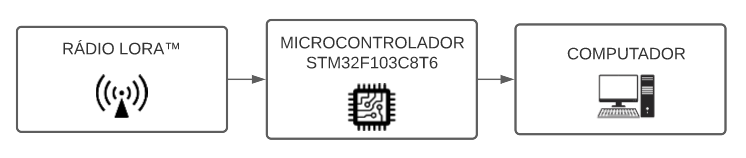
\includegraphics[width=1.0\textwidth]{img/Fluxograma_Sistema2.png}
    \end{center}
    \vspace{-0.5cm}
    \legend{\ABNTEXfontereduzida \textbf{Fonte: O autor.}}
    %\citeonline{BNO055}.}
    \label{fig:Fluxograma_Sistema2}
\end{figure}.
 

 
 
%######################################################################################## 
%######################################################################################## 
%######################################################################################## 

\section{Firmware} 



%####################################################################
%####################################################################
%####################################################################



Como o sistema a ser projetado tem a finalidade de obter dados de um objeto com altas velocidades. É de extrema importância conhecer os limites impostos por  componente, e assim, projetar um firmware capaz de extrair o máximo de cada componente. Com base no datasheet de cada sensor foi possível obter a taxa de atualização máxima e montar a tabela \ref{tempoderesposta_sensores}. 





\begin{table}[!thb]
	\centering
	\caption{\label{tempoderesposta_sensores}Tempo de resposta máxima dos sensores}
	\begin{tabular}{ll|c|c|}
		\cline{3-4}
		\multicolumn{1}{c}{\textbf{}} & 
		\multicolumn{1}{c|}{\textbf{}} & 
		\multicolumn{2}{l|}{\textbf{Taxa de atualização}} 
		\\ \cline{3-4}
		 & \multicolumn{1}{c|}{\textbf{}} & Hertz   & Milissegundos
		\\ \hline
		\multicolumn{1}{|c|}{\multirow{3}{*}{\textbf{Sensor BNO055}}} & Acelerômetro & $100$ & $10$ 
		\\ \cline{2-4}
		\multicolumn{1}{|l|}{} & Giroscópio & $100$ & $10$ 
		\\ \cline{2-4}
	    \multicolumn{1}{|l|}{} & Magnetrômetro & $20$ & $50$ 
		\\ \hline
		\multicolumn{1}{|c|}{\multirow{3}{*}{\textbf{Sensor BME280}}} & Barômetro & $25$ & $40$ 
		\\ \cline{2-4}
		\multicolumn{1}{|l|}{} & Umidade & $25$ & $40$ 
		\\ \cline{2-4}
	    \multicolumn{1}{|l|}{} & Temperatura & $25$ & $40$ 
		\\ \hline
		\multicolumn{1}{|c|}{\textbf{GPS NEO-6M}} & Geolocalização & $5$ & $200$ 
		\\ \hline
	\end{tabular}
	\Ididthis
\end{table}

%####################################################################
%####################################################################
%####################################################################

Através da tabela \ref{tempoderesposta_sensores}, é possível identificar que o GPS é o componente de entrada com maior lentidão, chegando a ser $20$ vezes mais lento do que o acelerômetro. Portanto, para uma leitura sequencial dos sensores, o GPS é o gargalo na entrada do sistema, forçando o sistema a operar a taxa de atualização de $5 \ Hz$.


Porém, existe um outro fator a ser considerado que é o volume máximo de dados que a saída do sistema suporta, através do rádio e do cartão micro SD. Como o cartão micro SD de menor classe (Classe 2) trabalha com pelo menos 2 MB/s (megabytes por segundo), este não afetará o sistema. Mas, segundo o datasheet do Rádio Lora, a taxa de envio padrão que o modulo consegue enviar é de $2,4 \ kbps$ ou $300 \ Bytes/s $, sendo bastante inferior ao cartão. De acordo com a tabela \ref{Tamanho_Variavel}, que mostra o volume total das variáveis a serem enviadas e com o valor máximo que o rádio suporta, temos que:


\begin{equation}
    \textbf{Taxa de atualização do rádio} = \frac{300}{72} = 4,16 \approx 4 \ Hz
\end{equation}


 Então o gargalo do sistema não será pelo GPS, mas sim, na saída dos dados pelo rádio. Limitando o sistema a operar em uma taxa máxima de $4$ ciclos de dados por segundo ou $250$ milissegundo por ciclo.











\begin{table}[!thb]
	\centering
	\caption{\label{Tamanho_Variavel}Variáveis do sistema}
	\begin{tabular}{ll|c|c|}
		\\ \cline{3-4}
		 & \multicolumn{1}{c|}{\textbf{}} & \textbf{Tipo}   & \textbf{Bytes} 
		\\ \hline
		\multicolumn{1}{|c|}{\multirow{3}{*}{\textbf{Acelerômetro}}} & X & Float & $4$ 
		\\ \cline{2-4}
		\multicolumn{1}{|l|}{} & Y & Float & $4$ 
		\\ \cline{2-4}
	    \multicolumn{1}{|l|}{} & Z & Float & $4$ 
		\\ \hline
		
		\multicolumn{1}{|c|}{\multirow{3}{*}{\textbf{Giroscópio}}} & X & Float & $4$  
		\\ \cline{2-4}
		\multicolumn{1}{|l|}{} & Y & Float & $4$ 
		\\ \cline{2-4}
	    \multicolumn{1}{|l|}{} & Z & Float & $4$ 
		\\ \hline	

		\multicolumn{1}{|c|}{\multirow{3}{*}{\textbf{Magnetômetro}}} & X & Float & $4$  
		\\ \cline{2-4}
		\multicolumn{1}{|l|}{} & Y & Float & $4$ 
		\\ \cline{2-4}
	    \multicolumn{1}{|l|}{} & Z & Float & $4$ 
		\\ \hline			
		
		\multicolumn{1}{|c|}{\textbf{Barômetro}} & A & Float & $4$ 
		\\ \hline

		\multicolumn{1}{|c|}{\textbf{Umidade}} & U & Float & $4$ 
		\\ \hline		
		
		\multicolumn{1}{|c|}{\textbf{Temperatura}} & T & Float & $4$ 
		\\ \hline		

		\multicolumn{1}{|c|}{\multirow{3}{*}{\textbf{GPS}}} & Latitude & Float & $4$  
		\\ \cline{2-4}
		\multicolumn{1}{|l|}{} & Longitude & Float & $4$ 
		\\ \cline{2-4}
		
	    \multicolumn{1}{|l|}{} & Altitude & Float & $4$ 
		\\ \cline{2-4}
	    \multicolumn{1}{|l|}{} & Velocidade & Float & $4$ 
		\\ \cline{2-4}
		
	    \multicolumn{1}{|l|}{} & Satélites & Int & $4$ 
		\\ \cline{2-4}		
		
	    \multicolumn{1}{|l|}{} & Horário & Unsigned long & $4$ 
		\\ \hline		
		
		\\ \cline{3-4}
		 & \multicolumn{1}{c|}{\textbf{}} & \textbf{Total}   & \textbf{72} 
		\\ \cline{3-4}
	\end{tabular}
	\Ididthis
\end{table}





















%####################################################################
%####################################################################
%####################################################################


\subsection{Firmware transmissor}





Como o sistema estará limitado em uma taxa de 250 milissegundos por ciclo, devido ao gargalo na saída do sistema, não será possível adicionar buffers para os sensores com maior taxa de atualização, e aproveitar os dados gerados no intervalo dos sensores de maior latência, por isso, o fluxo do firmware será sequencial como mostra a figura \ref{fig:Fluxograma_firmware1}. 










\begin{figure}[ht]
    \centering
    \caption{Fluxograma firmware do sistema contido no foguete.}
    \begin{center}
        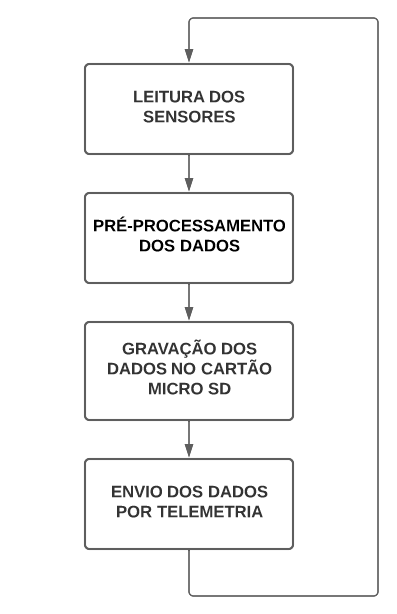
\includegraphics[width=0.50\textwidth]{img/Fluxograma_Firmware1.png}
    \end{center}
    \vspace{-0.5cm}
    \legend{\ABNTEXfontereduzida \textbf{Fonte: O autor.}}
    %\citeonline{BNO055}.}
    \label{fig:Fluxograma_firmware1}
\end{figure}.

\newpage

\subsection{Firmware Receptor}

 Por se tratar de  um sistema cuja finalidade é apenas receber os dados do foguete e enviar os dados para um computador, o firmware do receptor é mais simples do que o firmware do transmissor como é mostrado na figura \ref{fig:Fluxograma_firmware2}.




\begin{figure}[ht]
    \centering
    \caption{Fluxograma firmware do sistema no solo.}
    \begin{center}
        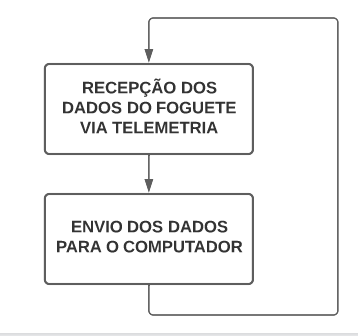
\includegraphics[width=0.45\textwidth]{img/Fluxograma_Firmware2.png}
    \end{center}
    \vspace{-0.5cm}
    \legend{\ABNTEXfontereduzida \textbf{Fonte: O autor.}}
    %\citeonline{BNO055}.}
    \label{fig:Fluxograma_firmware2}
\end{figure}.
 
 
 


\newpage



\section{Viabilidade econômica}

 A viabilidade econômica é um fator importante para este projeto, visto que o recurso financeiro obtido pela equipe tem como origem principal as doações pessoais. Então, todos os componentes foram escolhidos tendo em vista o melhor custo-benefício. O orçamento foi realizado para o sistema embarcado do foguete mostrado na tabela \ref{tab:Orçamento1}, para o sistema em solo mostrado na tabela \ref{tab:Orçamento2} e por fim o valor total do projeto visto na tabela \ref{tab:Orçamento3}.


 


\begin{table}[!thb]
	\centering
	\caption{Preço dos componentes para o sistema embarcado do foguete em 21/03/2022.}
    \begin{adjustbox}{max width={\textwidth},keepaspectratio}%
	\begin{tabular}{|ll|c|c|}
		\cline{3-4}
		\multicolumn{1}{c}{\textbf{}} & 
		\multicolumn{1}{c|}{\textbf{}} & 
		\multicolumn{2}{l|}{\textbf{Preço + Frete}} 
		\\ \cline{1-4}
		 & \multicolumn{1}{c|}{\textbf{Componente}} & \textbf{(USD)} & \textbf{(BRL)}
		 \\ \hline
		& \multicolumn{1}{c|}{STM32F103C8} & 6.92 & 36,47
		 \\ \hline
        & \multicolumn{1}{c|}{V2 Link} & 6.92 & 36,47
		 \\ \hline
        & \multicolumn{1}{c|}{ GPS NEO-6M } & 8.33 & 43,56
		 \\ \hline
        & \multicolumn{1}{c|}{Sensor BNO055} & 39.49 & 208,13
		 \\ \hline
        & \multicolumn{1}{c|}{Sensor BME280} & 9.59 & 50,46
		 \\ \hline
        & \multicolumn{1}{c|}{Radio Lora } & 20.72 & 66,04
		 \\ \hline
        & \multicolumn{1}{c|}{2 Antena radio lora} & 8.00 & 41,53
		 \\ \hline
		 
		 
		 
		 
		 & \multicolumn{1}{c|}{\textbf{Total}} & \textbf{99.97} & \textbf{482,66}
		 \\ \hline

	\end{tabular}
    \end{adjustbox}
%	\Ididthis
	\legend{\ABNTEXfontereduzida \textbf{Fonte:} O autor.}
    \label{tab:Orçamento1} 
\end{table}



Devido a escassez de circuitos eletrônicos e ao aumento do dólar de 4,30 em 11/02/2020 para 5,02  em 2022 causado pela pandemia alguns dos sensores ficaram bastante caros comparado com o valor adquirido no ano de 2020, como é o caso do sensor BNO055 que foi adquirido por 7.22 dólares em 2020 e no ano de 2022 está por 39.49 dólares.  











\begin{table}[!thb]
	\centering
	\caption{Preço dos componentes para o sistema embarcado em solo em 21/03/2022.}
    \begin{adjustbox}{max width={\textwidth},keepaspectratio}%
	\begin{tabular}{|ll|c|c|}
		\cline{3-4}
		\multicolumn{1}{c}{\textbf{}} & 
		\multicolumn{1}{c|}{\textbf{}} & 
		\multicolumn{2}{l|}{\textbf{Preço + Frete}} 
		\\ \cline{1-4}
		 & \multicolumn{1}{c|}{\textbf{Componente}} & \textbf{(USD)} & \textbf{(BRL)}
		 \\ \hline
		& \multicolumn{1}{c|}{STM32F103C8} & 6.92 & 36,47
		 \\ \hline
        & \multicolumn{1}{c|}{Radio Lora } & 20.72 & 66,04
		 \\ \hline

		 
		 
		 
		 
		 & \multicolumn{1}{c|}{\textbf{Total}} & \textbf{27.64} & \textbf{102,51}
		 \\ \hline

	\end{tabular}
    \end{adjustbox}
%	\Ididthis
	\legend{\ABNTEXfontereduzida \textbf{Fonte:} O autor.}
    \label{tab:Orçamento2} 
\end{table}






\begin{table}[!thb]
	\centering
	\caption{Preço total dos sistemas em 21/03/2022.}
    \begin{adjustbox}{max width={\textwidth},keepaspectratio}%
	\begin{tabular}{|ll|c|c|}
		\cline{3-4}
		\multicolumn{1}{c}{\textbf{}} & 
		\multicolumn{1}{c|}{\textbf{}} & 
		\multicolumn{2}{l|}{\textbf{Preço + Frete}} 
		\\ \cline{1-4}
		 & \multicolumn{1}{c|}{\textbf{Componente}} & \textbf{(USD)} & \textbf{(BRL)}
		 \\ \hline
		& \multicolumn{1}{c|}{Sistema embarcado do foguete} & 99.97 & 482,66
		 \\ \hline
        & \multicolumn{1}{c|}{Sistema embarcado em solo } & 27.64 & 102,51
		 \\ \hline

		 
		 
		 
		 
		 & \multicolumn{1}{c|}{\textbf{Total}} & \textbf{127.61} & \textbf{585,17}
		 \\ \hline

	\end{tabular}
    \end{adjustbox}
%	\Ididthis
	\legend{\ABNTEXfontereduzida \textbf{Fonte:} O autor.}
    \label{tab:Orçamento3} 
\end{table}


















\begin{comment}
\begin{table}[!thb]
	%\huge
    \centering
    \caption{Preço dos componentes a serem utilizados 21/03/2022.}
    \begin{adjustbox}{max width={\textwidth},keepaspectratio}%
    \begin{tabular}{@{} p{6.5cm}|c|c|c| }
        \toprule
        \textbf{Componente}
        & Preço incluindo frete (USD) & 
        \\ \hline
        STM32F103C8
        & 6.92   &   36,47   
        \\ \hline
        V2 Link
        & 6.92   &  36,47  
        \\ \hline
        GPS NEO-6M 
        & 8.33   & 43,56
        \\
        \bottomrule
    \end{tabular}
    \end{adjustbox}
    \legend{\ABNTEXfontereduzida \textbf{Fonte:} O autor.}
    \label{tab:cronograma} 
    % \legend{\textbf{Fonte:} O autor.}
\end{table}

\end{comment}






%--------------------------------------------------------------------------------------
% Insere a seção de cronograma
%--------------------------------------------------------------------------------------



\newpage



\section{Cronograma} 
\label{sec:crono}

%A tabela \ref{tab:cronograma} mostra o cronograma de atividades a serem executadas para o TCC II, com base no calendário de 201X.Y da UNIVASF.

A Tabela \ref{tab:cronograma} mostra o cronograma de atividades a serem executadas para o Trabalho de Conclusão II (TCC II), com base no calendário do período 2021.2 da UNIVASF, definido pelo Calendário Acadêmico 2021 da instituição.

\begin{table}[!thb]
	%\huge
    \centering
    \caption{Cronograma das atividades previstas para o TCC II.}
    \begin{adjustbox}{max width={\textwidth},keepaspectratio}%
    \begin{tabular}{@{} p{6.5cm}|c|c|c|c|c|c @{}}
        \toprule
        \textbf{Atividade}
        & Mai & Jun & Jul & Ago & Set & Out
        \\ \hline
        Teste dos sensores individualmente em bancada 
        & X   &     &     &     &     &          
        \\ \hline
        Teste do modulo de Telemetria em bancada
        & X   &     &     &     &     &          
        \\ \hline
        Desenvolvimento da PCB
        &    & X   & X    &     &     &          
        \\ \hline
        Teste completo da PCB em bancada
        &     &    & X   &     &     &          
        \\ \hline
        Teste do sistema em um minifoguete 
        &     &    &    & X    &     &    
        \\ \hline
        Escrita do TCC II                       
        & X   & X   & X   & X   &    &         
        \\ \hline
        Defesa do TCC II                        
        &     &     &     &     & X   &        
        \\
        \bottomrule
    \end{tabular}
    \end{adjustbox}
    \legend{\ABNTEXfontereduzida \textbf{Fonte:} O autor.}
    \label{tab:cronograma} 
    % \legend{\textbf{Fonte:} O autor.}
\end{table}

